\documentclass[11pt, a4paper,titlepage]{article}
\usepackage[utf8]{inputenc}
\usepackage{setspace}
\usepackage{longtable}
\usepackage{textpos}
\usepackage{acronym}
\usepackage[nonumberlist,acronym,toc]{glossaries}
\usepackage{latexsym}
\usepackage{textcomp}
\usepackage[bottom]{footmisc}
\usepackage[left=2.85cm, right=2.85cm, top=2cm, bottom=2cm]{geometry}
\usepackage[english]{babel}
\usepackage{graphicx}
\graphicspath{ {figures/} }
\usepackage{array}
\usepackage{float}
\usepackage{pdfpages}
\usepackage{titlesec}
\usepackage{siunitx}
\usepackage{enumitem}
\usepackage{adjustbox}
\usepackage[small]{caption}
\usepackage{subcaption}
\usepackage{listings}
\usepackage{lscape}
\usepackage[toc,page]{appendix}
\usepackage[pdftex, pdfborderstyle={/S/U/W 0} % this disables the boxes around links
            ]{hyperref}
\usepackage{color}
\lstset{ %
  language=R,                % the language of the code
  basicstyle=\footnotesize,           % the size of the fonts that are used for the code
  numbers=left,                   % where to put the line-numbers
  numberstyle=\tiny\color{gray},  % the style that is used for the line-numbers
  stepnumber=1,                   % the step between two line-numbers. If it's 1, each line
                                  % will be numbered
  numbersep=5pt,                  % how far the line-numbers are from the code
  backgroundcolor=\color{white},      % choose the background color. You must add \usepackage{color}
  showspaces=false,               % show spaces adding particular underscores
  showstringspaces=false,         % underline spaces within strings
  showtabs=false,                 % show tabs within strings adding particular underscores
  %frame=single,                   % adds a frame around the code
  rulecolor=\color{black},        % if not set, the frame-color may be changed on line-breaks within not-black text (e.g. commens (green here))
  tabsize=2,                      % sets default tabsize to 2 spaces
  captionpos=b,                   % sets the caption-position to bottom
  breaklines=true,                % sets automatic line breaking
  breakatwhitespace=false,        % sets if automatic breaks should only happen at whitespace
  title=\lstname,                   % show the filename of files included with \lstinputlisting;
                                  % also try caption instead of title
  keywordstyle=\color{blue},          % keyword style
  commentstyle=\color{gray},       % comment style
  stringstyle=\color{purple},         % string literal style
  %escapeinside={\%*}{*)},            % if you want to add a comment within your code
  morekeywords={*,...}               % if you want to add more keywords to the set
}

% Equation environment
\newenvironment{conditions}
  {\par\vspace{\abovedisplayskip}\noindent\begin{tabular}{>{$}l<{$} @{${}={}$} l}}
  {\end{tabular}\par\vspace{\belowdisplayskip}}

\begin{document}

\begin{titlepage}
  \begin{center}
    
    
\includegraphics[scale=1.5]{figures/kuleuven_logo.pdf}~\\[4.5cm]
    \textsc{\Large Master of bioinformatics}\\[0.5cm]

    % Title
    \rule{\linewidth}{0.3mm}\\[0.4cm]
    {\huge \bfseries Applied multivariate statistical analysis} \\[0.4cm]
    {\large Multivariate dataset exploration: genome assembly} \\[0.4cm]
    \rule{\linewidth}{0.3mm}\\[0.4cm]
    {\large Summer 2016} \\[1.0cm]
    
    % Author and supervisor
    \begin{minipage}{0.4\textwidth}
      \begin{flushleft} \large
        \emph{Author:}\\
	Cedric \textsc{Lood}
      \end{flushleft}
    \end{minipage}
%     %\hfill
    \begin{minipage}{0.4\textwidth}
      \vspace{25pt}
      \begin{flushright} \large
        \emph{Teacher:} \\
        Prof. Eddie \textsc{Schrevens}\\
        \hfill \newline 
      \end{flushright}
    \end{minipage}
    
    \vfill

    
\includegraphics[scale=0.15]{figures/KUL.jpg}~\\[0cm]

    % Bottom of the page
    {\large \today}
    
  \end{center}
\end{titlepage}


\section{Context of this project}

The analysis presented in this report was produced for the class of
\emph{Applied multivariate statistics} taught at KU Leuven (Winter
2015). The requirement for the class included the exploration of a
multivariate dataset of our choice in order to discover its
structure. The implementation was done using the R programming
environment (v3.3.0), and the dataset along with the code can be found
online in my github
account\footnote{https://github.com/Milt0n/MVDataExploration}.

\section{Genome assembly: quality control metrics}

The dataset consists of quality control metrics for \emph{de novo}
genome assembly \cite{baker2012novo}. It originates from an analysis
performed in the early stages of my master thesis in which I
investigated the genomics of a set of 47 nosocomial isolates of the
bacterial species \emph{Pseudomonas aeruginosa}.

The goal of genome assembly is to reconstruct the genome of an
organism using the short reads issued by the sequencer, which in my
case was from \emph{Illumina}. Multiple genome assemblies were
performed using different software and approaches for each of my 47
strains. Each assembly gave slightly different hypothesis for what the
original sequenced genome was.

In this analysis, the goal is to detect outliers in order to remove
them from the set of hypothesis, and explore the structure of the data
in order to decide which variables can be used to select the best
hypothesis for each strains via an ensemble method.

\section{Description of the dataset}

The dataset consists of 36 variables and 3102 observations, as each of
the 47 strains went through 67 different assemblie. A few missing
values exist in the dataset, but their amount is very limited (43 out
of 3102) and can be traced back to software errors, hence they were
removed prior to the analysis. An exhaustive description of the
variables is available here \cite{gurevich2013quast}, here is a
summary of selected variables:

\begin{table}[h]
  \centering
  \begin{tabular}{|l|l|l|}
    \hline
    \# & name            & description                                                  \\ \hline
    1  & Strain ID       & Label with the ID of the strain (from 9108 to 9154)          \\
    2  & Assembly        & Label for the 67 assembly pipelines                          \\
    3  & Hybrid          & Boolean value indicating the approach for the assembly       \\ 
    4  & Coverage        & Genome coverage estimation based on sequencing results       \\
    5  & NContig         & Total number of contigs for the assembly                     \\
    6  & LargestContig   & Length (in base pairs) of the longuest contig                \\
    7  & TotalLength     & Total length of the assembled genome                         \\ 
    8  & ReferenceLength & Length of reference genome used for QC evaluation            \\ 
    9  & GC              & GC content of the assembled genome (\%)                      \\ 
    10 & ReferenceGC     & GC content of reference genome used for QC evaluation        \\
    11 & N50             & Minimum length of contig comprising 50\% of assembled genome \\ 
    12 & NG50            & Corrected N50 using the length of reference genome           \\ 
    13 & N75             & Minimum length of contig comprising 75\% of assembled genome \\ 
    15 & L50             & Number of contigs of length greater than N50                 \\ 
    19 & Nmisassemblies  & Number of misassemblies events                               \\ 
    24 & GenomeFraction  & Fraction of reference genome covered by assembly             \\ 
    29 & NA50            & Corrected N50 taking into account misassemblies              \\ 
    30 & NGA50           & Corrected NG50 taking into account misassemblies             \\ 
    36 & LGA75           & Corrected LG75 taking into account misassemblies             \\ \hline
  \end{tabular}
\end{table}

\section{Output}
\subsection{Dataset structure}

\begin{figure}[H]
  \centering
  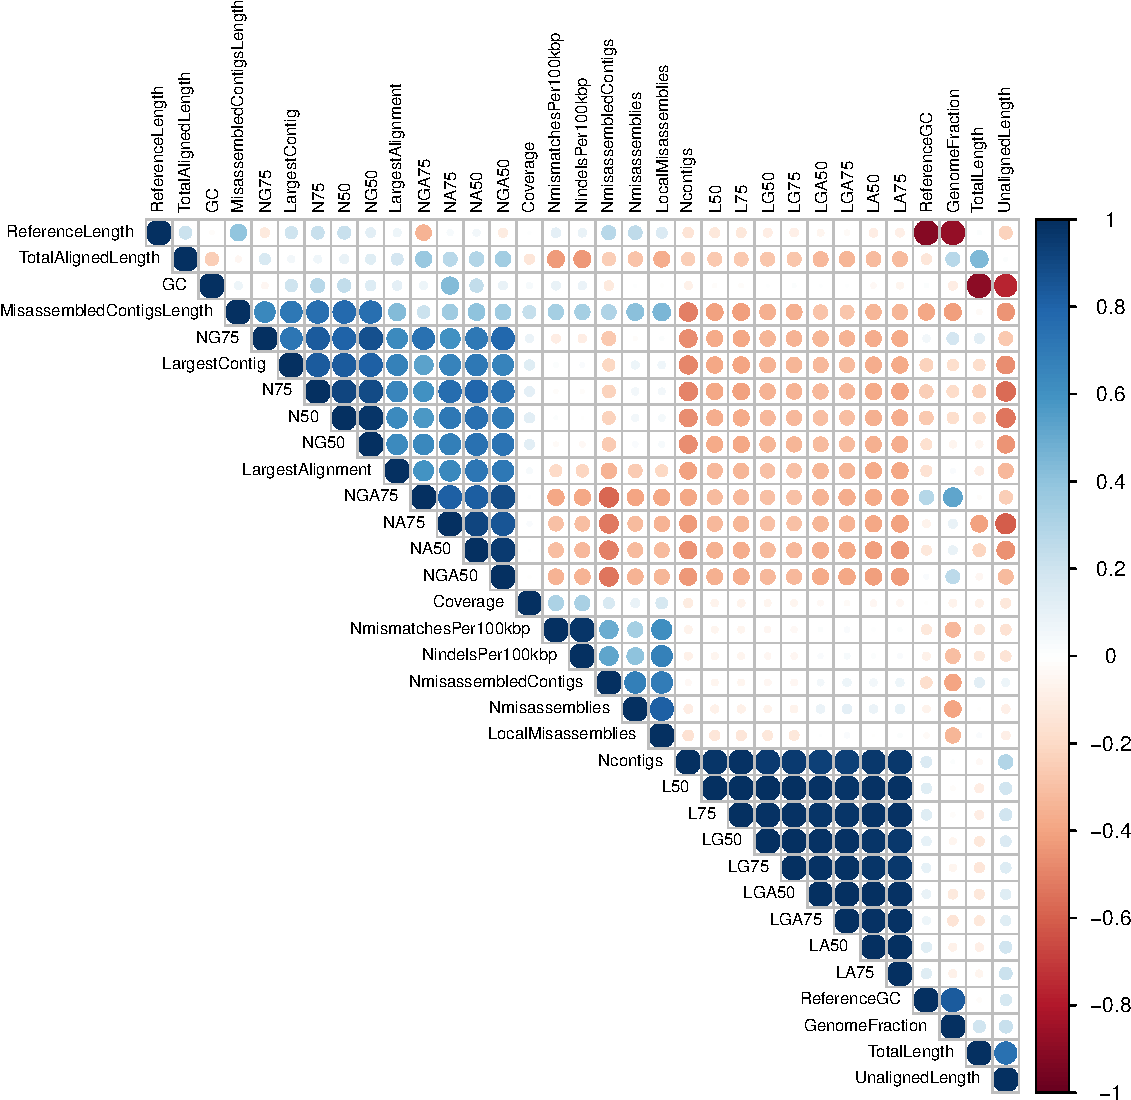
\includegraphics[scale=0.6]{corrplot.pdf}
  \caption{This graph shows the correlation between the different
    variables of the dataset, from a correlation of +1 (blue) to -1
    (red)}
  \label{fig:corrplot}
  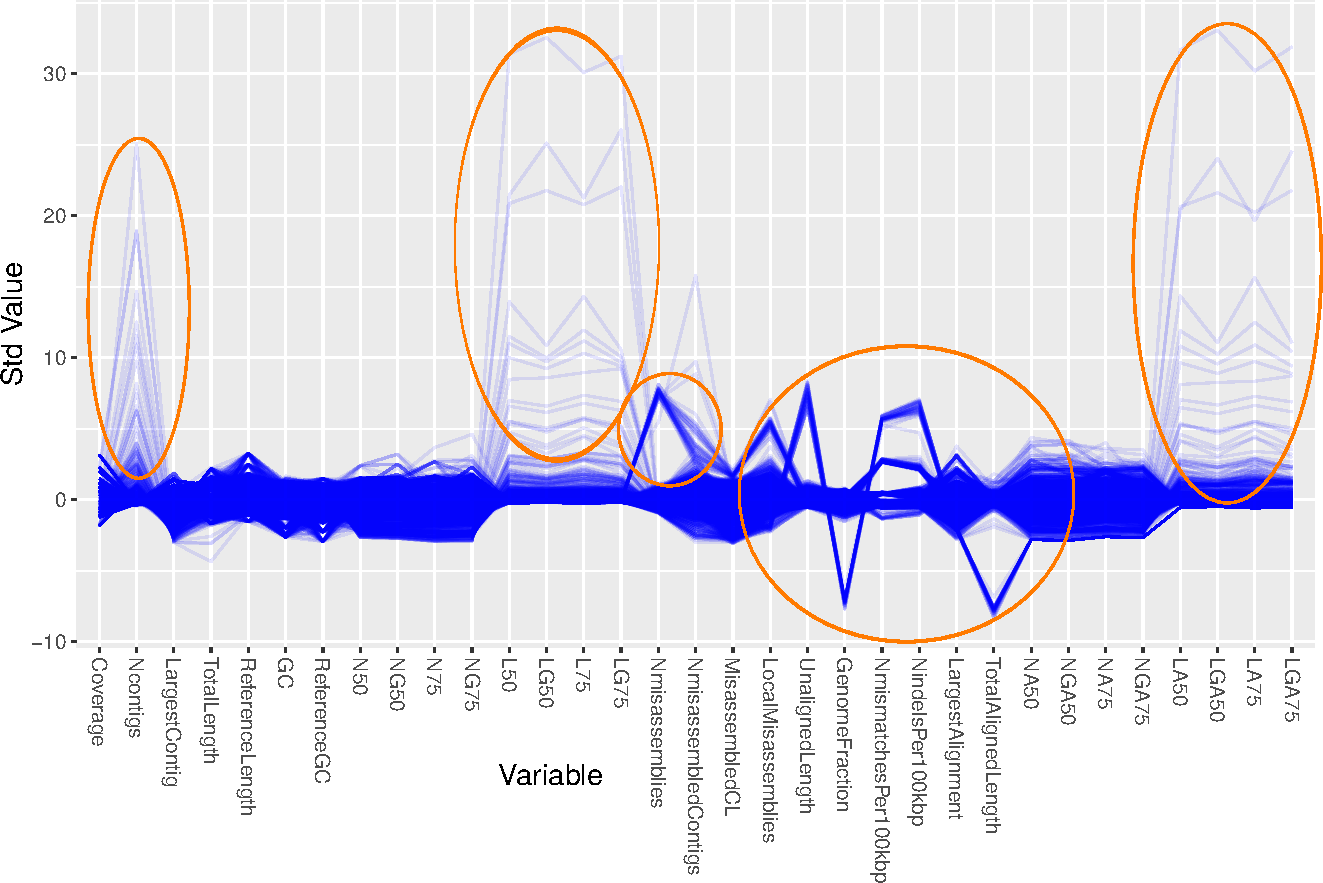
\includegraphics[scale=0.6]{parcoord.pdf}
  \caption{Parallel coordinates plot showing strong outliers (circled
    in orange)}
  \label{fig:parcoord}
\end{figure}

\begin{figure}[h]
  \begin{subfigure}{.5\textwidth}
    \centering
    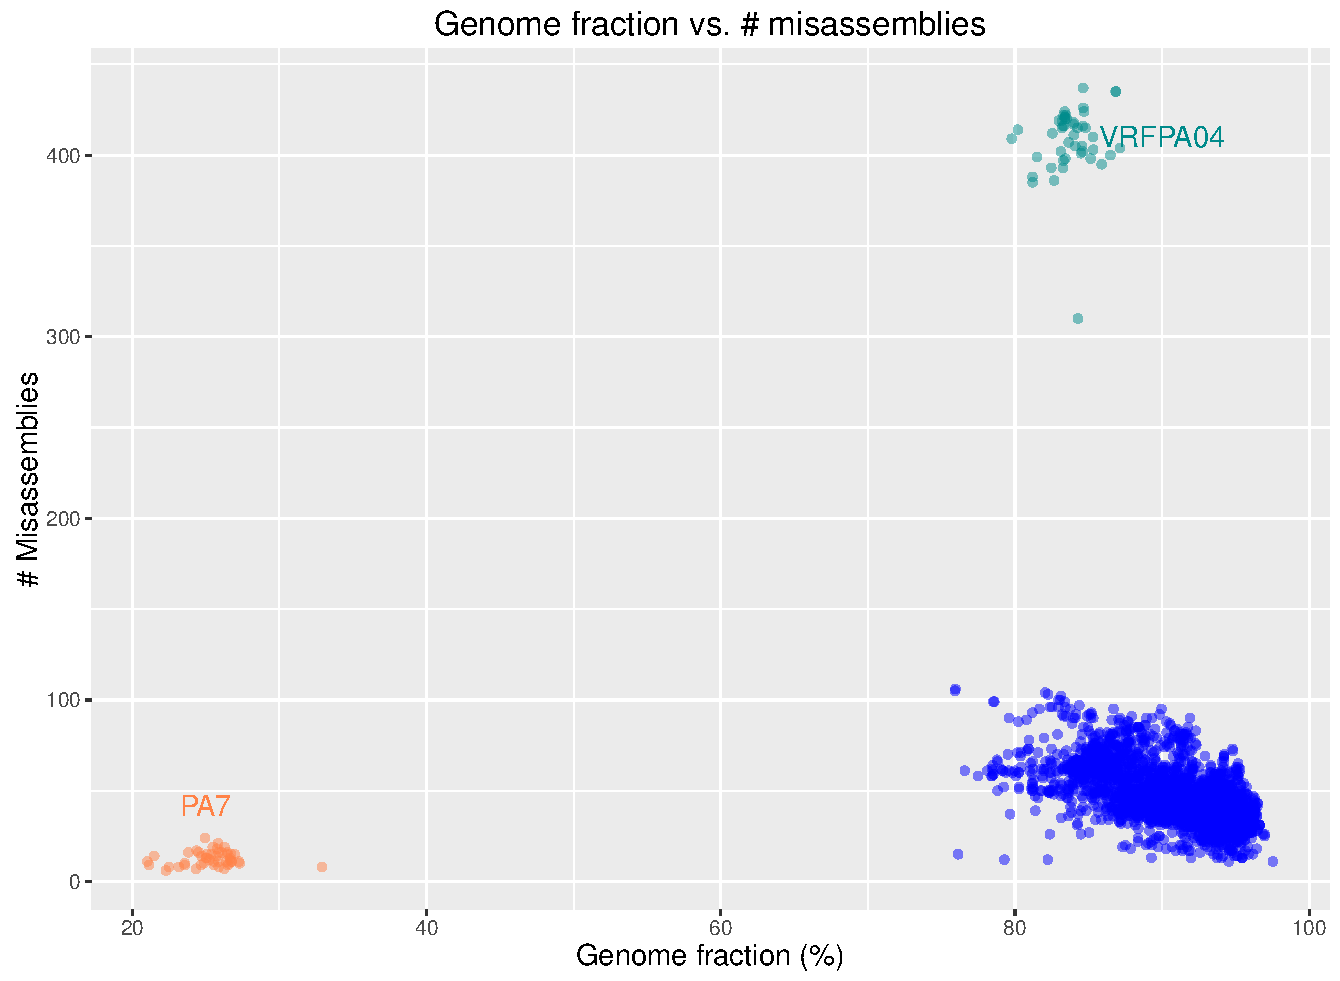
\includegraphics[width=1\linewidth]{scatterplot_gfvsmis.pdf}
  \end{subfigure}%
  \begin{subfigure}{.5\textwidth}
    \centering
    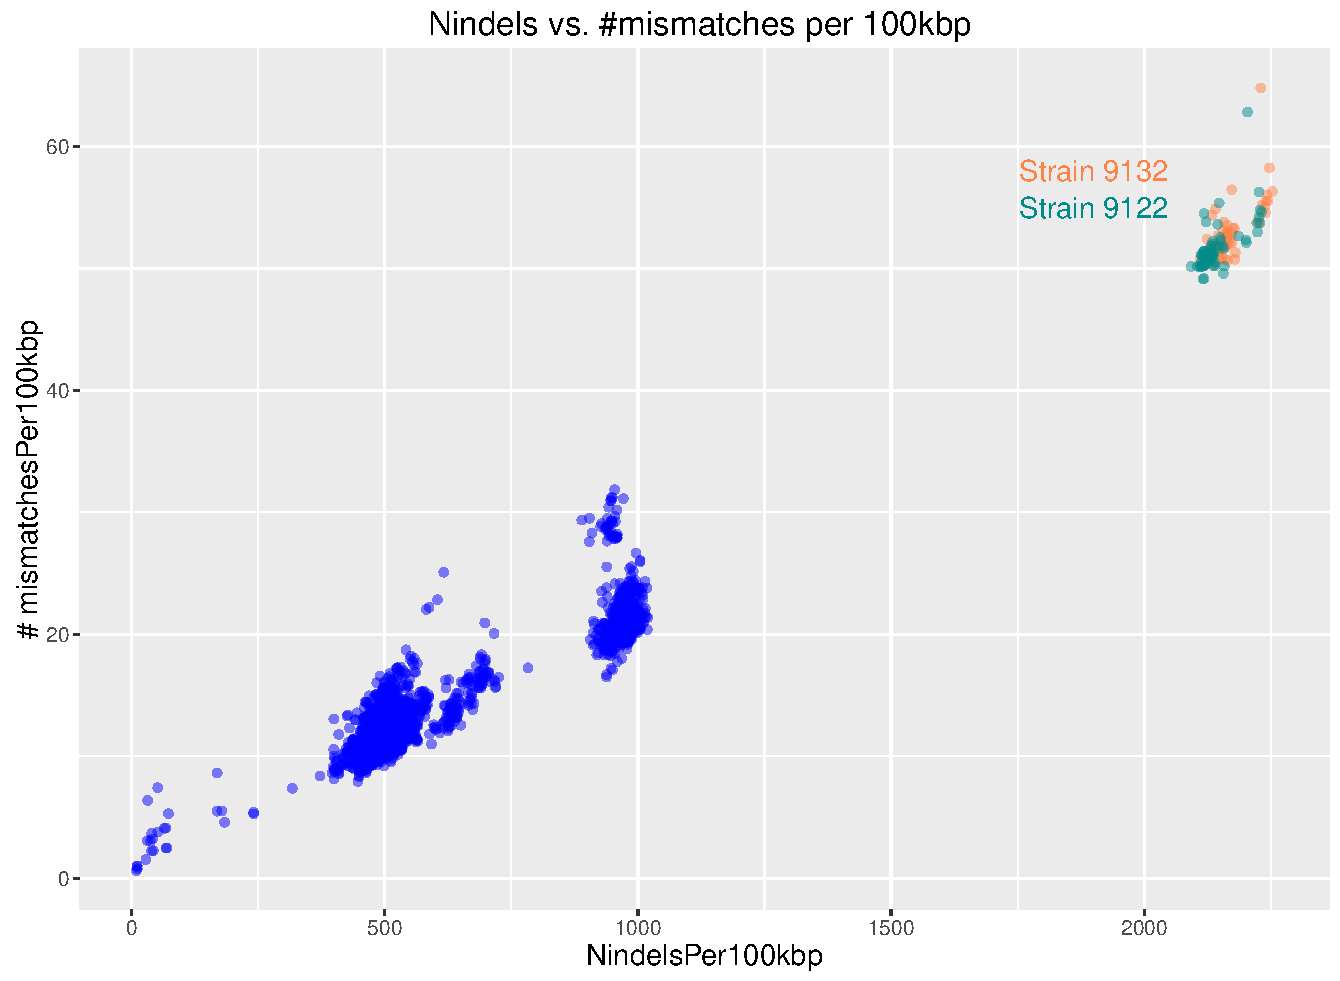
\includegraphics[width=1\linewidth]{scatterplot_indels.pdf}
  \end{subfigure}
  \caption{Outlier clusters detected and removed from the set of
    hypothesis}
  \label{fig:outliers}
\end{figure}

\begin{figure}[h]
  \begin{subfigure}{.5\textwidth}
    \centering
    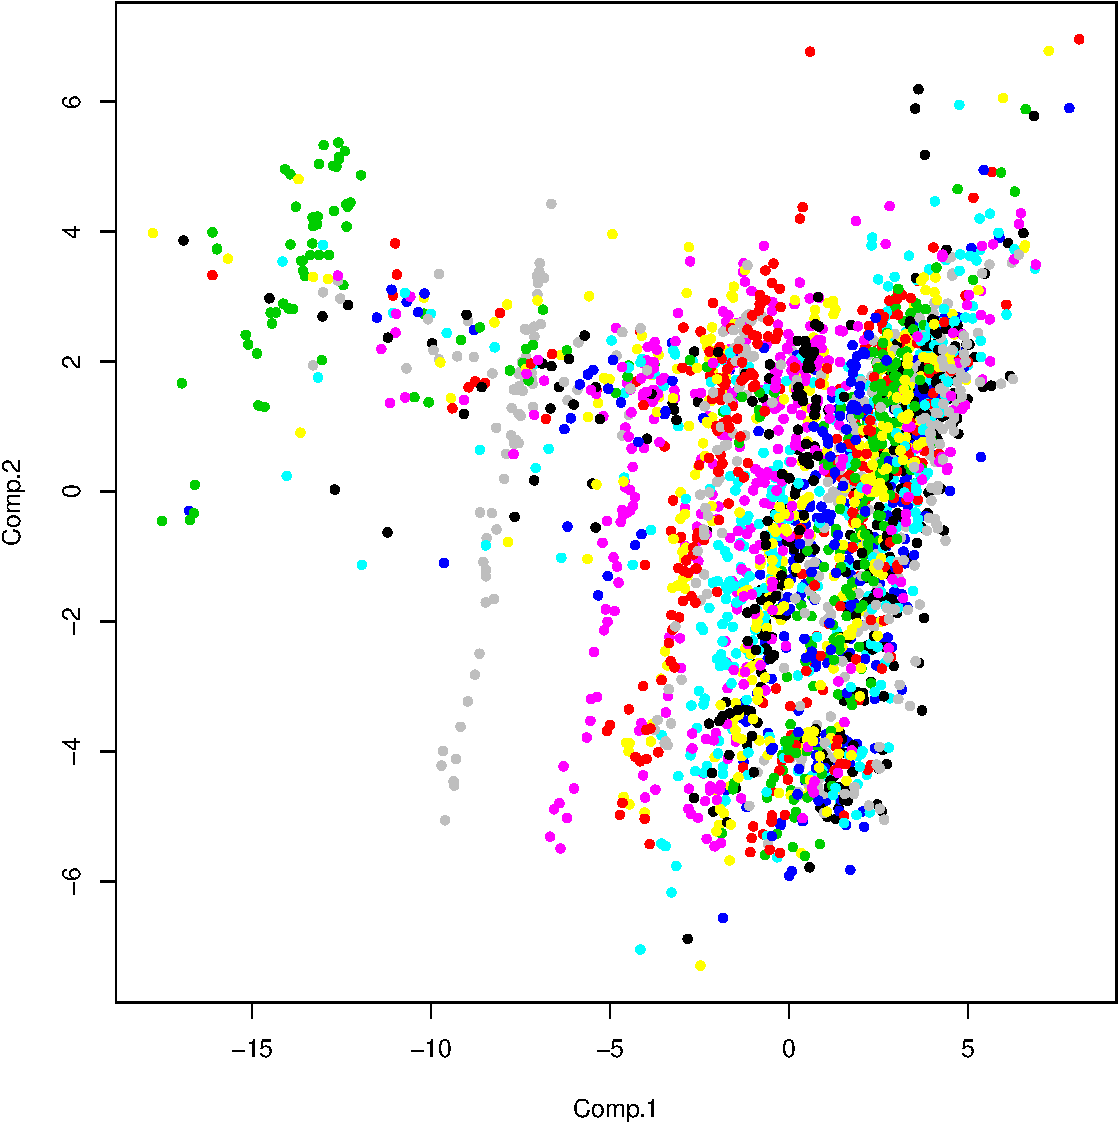
\includegraphics[width=1\linewidth]{pca.pdf}
  \end{subfigure}%
  \begin{subfigure}{.5\textwidth}
    \centering
    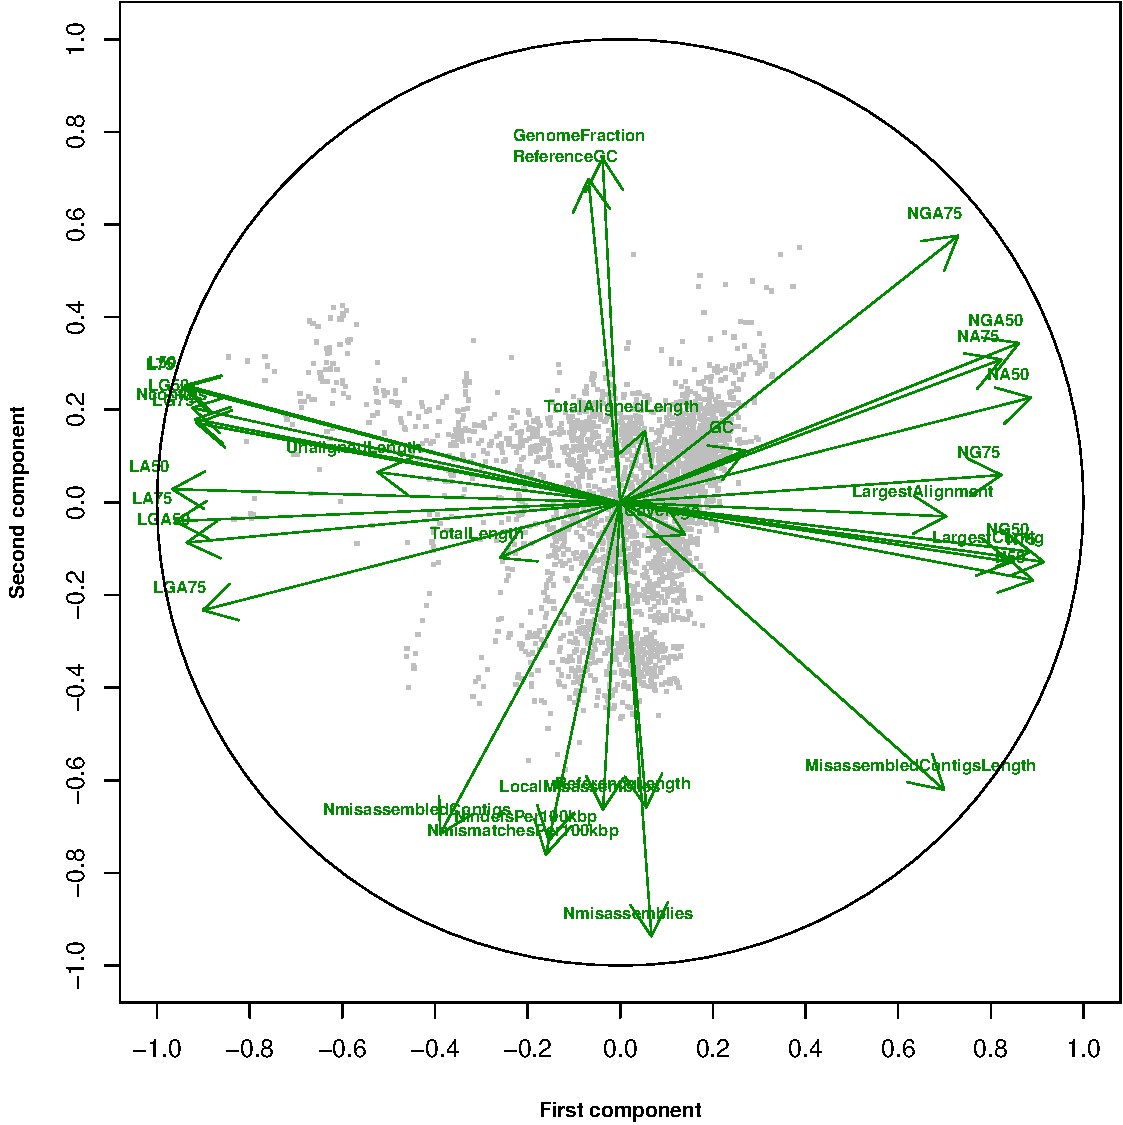
\includegraphics[width=1\linewidth]{biplot.pdf}
  \end{subfigure}
  \caption{left: Scores plot for the first 2 PC, coloured by strains;
    right: biplot graph.}
  \label{fig:pcplot}
\end{figure}

\begin{figure}[h]
  \begin{subfigure}{.5\textwidth}
    \centering
    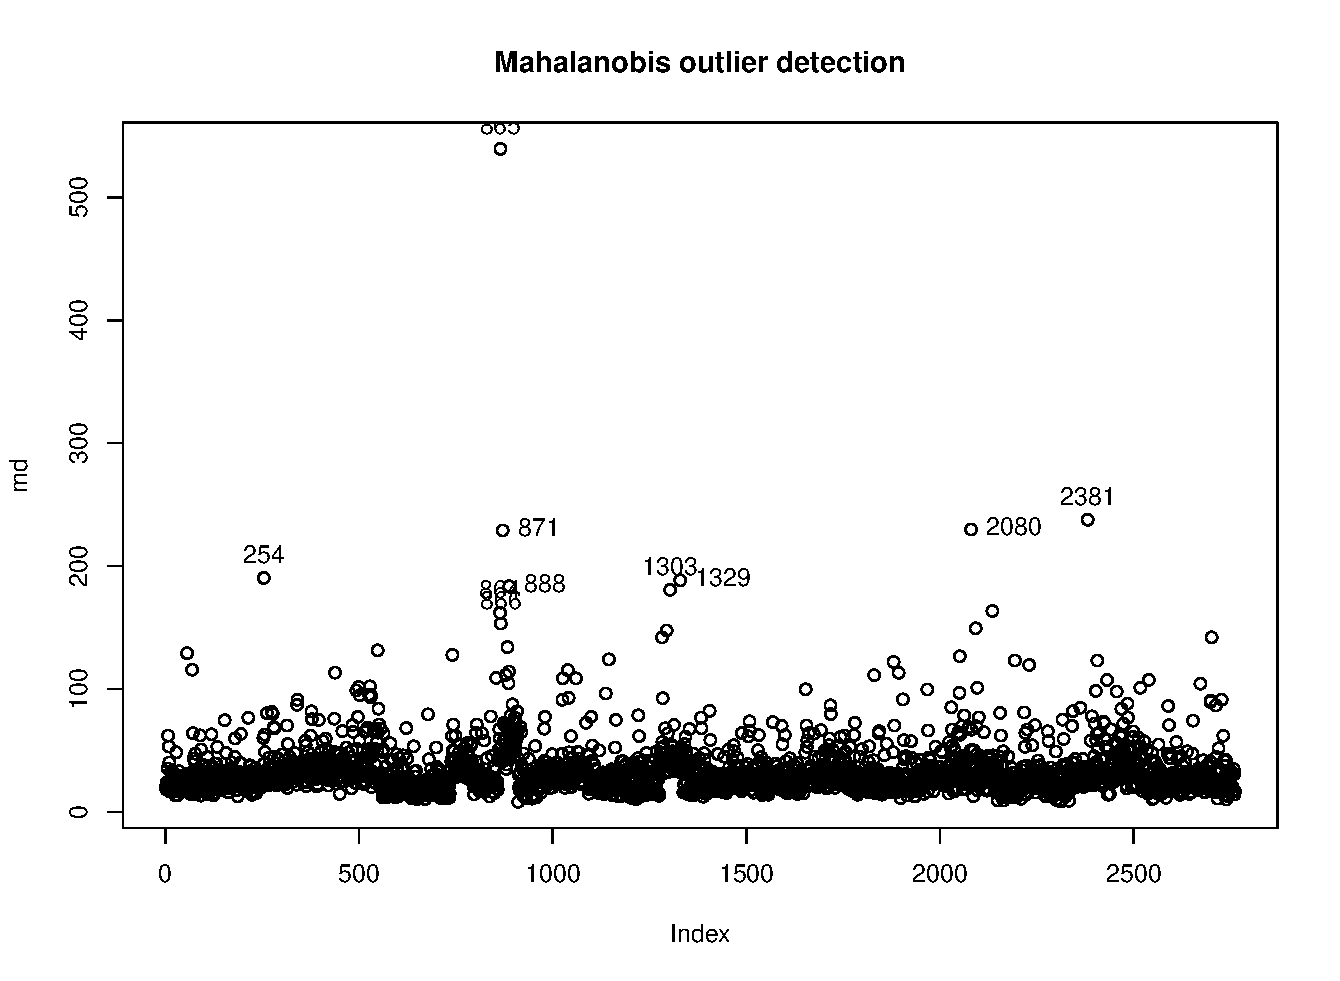
\includegraphics[width=1\linewidth]{mahalanobis.pdf}
  \end{subfigure}%
  \begin{subfigure}{.5\textwidth}
    \centering
    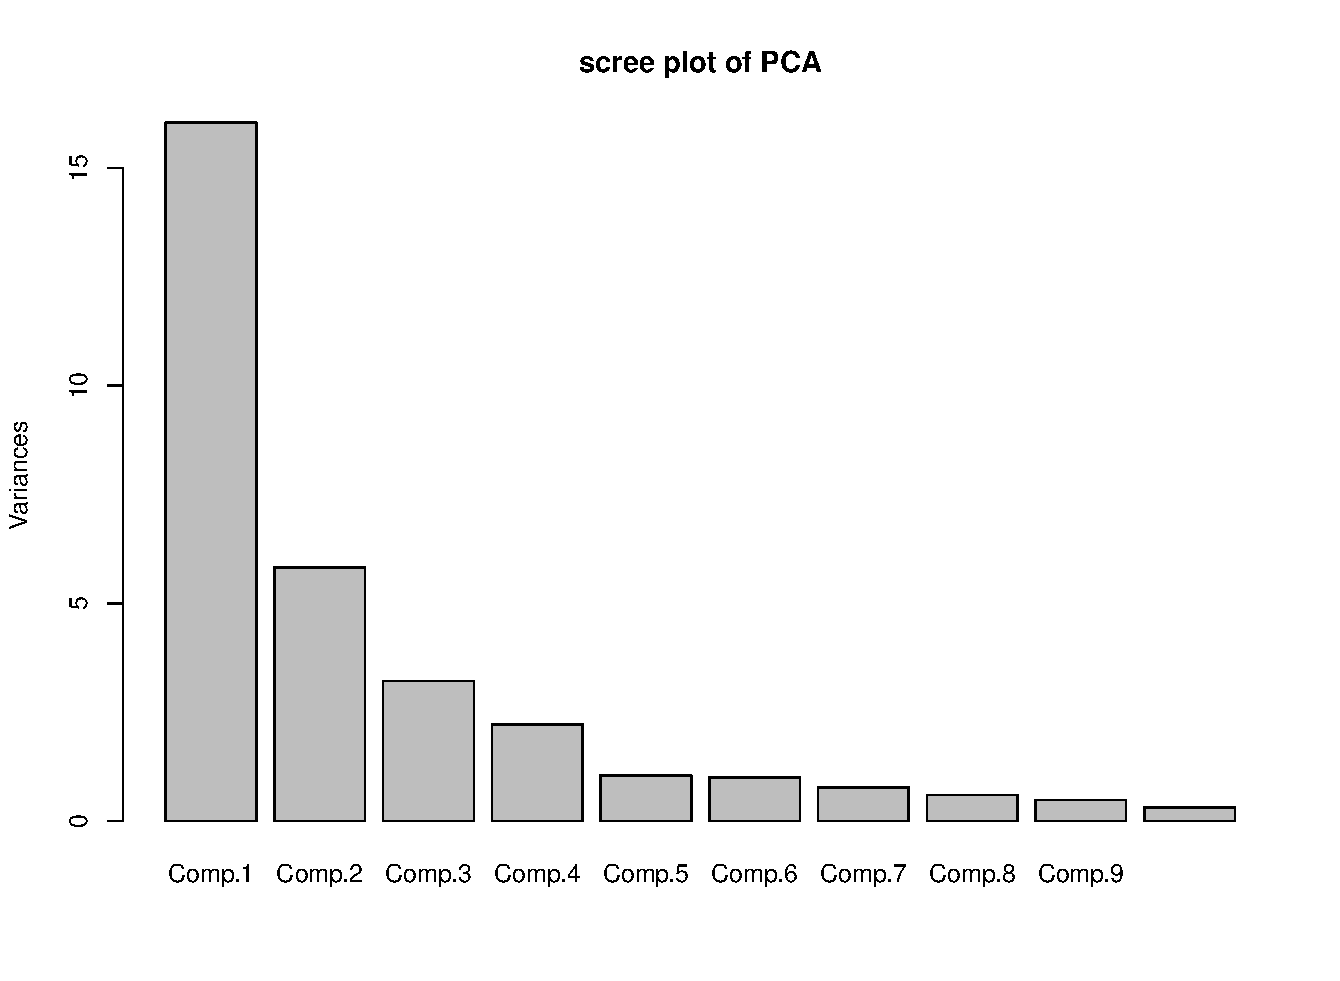
\includegraphics[width=1\linewidth]{screeplot.pdf}
  \end{subfigure}
  \caption{Left: mahalanobis plot and outliers identification, right: PCA scree plot}
\end{figure}

\section{Interpretation}

The dataset displays a lot of correlational structure in many of the
variables, as illustrated on figure \ref{fig:corrplot}. Looking into
the definition of the metrics helped understand why that is. The
parallel coordinates plot (figure \ref{fig:parcoord}) allowed
identification of many outlier clusters which were investigated
further and are illustrated on figure \ref{fig:outliers}. A biological
explanation was discovered for the presence of these clusters, and
they were eliminated from the list of hypothesis.

Given the existence of correlational structure, PCA was used here to
uncover the real dimensionality of the dataset. The analysis was based
on the correlation matrix because of huge scale differences accross
the variables. A large amount of variability can be captured using PCs
(the first 7 PCs explain 91\% of the variability, and 10 PCs
explaining 96\%). The plot and biplot of the two first component
(figure \ref{fig:pcplot}) showed an interesting line grouping
structure, with the colors indicating the different strains, this
grouping structure was also partially captured during attempts at
hierarchical clustering. Factor analysis (code not reported here)
showed a large amount of commonality using a few factors.

The analysis presented here was also combined with some other
univariate exploration of the variables, such as GC content, length of
assembly, etc. and it allowed me to filter out a fair amount of
outlier hypothesis. In the end, the metric NGA50 proved to be the most
interesting to make my ensemble decision upon.

\section{R Code}

Some of the ggplot code has been truncated (themes and
annotations). The full code is available in my github repository,
together with other attempts at analysis (factor analysis,
clustering):

\begin{lstlisting}[language=R]
library(ggplot2)
library(corrplot)
library(pastecs)
library(plotrix)
library(rgl)

setwd(dir = "/home/sid/Dev/MVDataExploration/data/")
asm <- read.csv(file = "quast_all_metrics_reduced.csv", header=TRUE)
str(asm); dim(asm)

# basic dataset statistics, correlations
stat.desc(asm[,4:36], basic=TRUE, desc=TRUE)
asm.corr <- cor(asm[,4:36])
corrplot(asm.corr, type="upper", order="hclust", tl.col="black", tl.srt=90)

# Profile plot 
asm.matrix <- as.matrix(asm[,4:36]) 
asm.matrix.std <- scale(asm.matrix, center=T, scale=T) 
asm.melt <- melt(asm.matrix.std)
colnames(asm.melt) <- c("RowID", "Variable", "Value")

ggplot(asm.melt,aes(x=Variable,y=Value,group=RowID)) +
  geom_line(colour=I("blue"), alpha=0.1)

# outliers
ggplot(asm, aes(GenomeFraction, Nmisassemblies)) +
  geom_point(data=subset(asm, Assembly != "PA7" & Assembly != "VRFPA04"), colour=I("blue"),alpha=0.5) +
  geom_point(data=subset(asm, Assembly == "PA7"), colour=I("sienna1")) +
  geom_point(data=subset(asm, Assembly == "VRFPA04"), colour=I("cyan4"))
ggsave("scatterplot_gfvsmis.pdf")

# subsetting (removal of the 2 pipelines PA7 and VRFPA04, and Ncontigs > 400)
asm.filter <- subset(asm, Assembly != "PA7" & Assembly != "VRFPA04" & Ncontigs < 400)

ggplot(asm.filter, aes(NmismatchesPer100kbp, NindelsPer100kbp)) +
  geom_point(data=subset(asm.filter, StrainID != "9122" & StrainID != "9132"), colour=I("blue"),alpha=0.5) +
  geom_point(data=subset(asm.filter,StrainID == "9122"),colour=I("sienna1")) +
  geom_point(data=subset(asm.filter,StrainID == "9132"),colour=I("cyan4"))
ggsave("scatterplot_indels.pdf")

# further subsetting using mahalanobis
asm.filter <- subset(asm.filter, StrainID != "9122" & StrainID != "9132" & Ncontigs < 400)
md <- mahalanobis(asm.filter[,4:36], colMeans(asm.filter[,4:36]), cov(asm.filter[,4:36]))
plot(md, main="Mahalanobis outlier detection")
identify(md)
asm.filter <- asm.filter[-c(865,254,871,1329,2080,2381,888,1303,866,864),]

# PCA analysis
asm.pca <- princomp(asm.filter[,4:36], cor = T)
screeplot(asm.pca)
asm.pca$loadings
summary(asm.pca)
plot(asm.pca$scores[,1:2], type="p", pch=19, cex=0.7, col=asm.filter$StrainID)
plot3d(asm.pca$scores[,1:3], col=asm.filter$StrainID)

# biplot
asm.matrix <- as.matrix(asm.filter[,4:36])
xm<-apply(asm.matrix,2,mean)
y<-sweep(asm.matrix,2,xm)
ss<-(t(y)%*%y)
s<-ss/(nrow(x)-1)
d<-(diag(ss))^(-1/2)
e<-diag(d,nrow=ncol(asm.matrix),ncol=ncol(asm.matrix))
z<-y%*%e
r<-t(z)%*%z
q<-svd(z)
gfd<-((q$d[1])+(q$d[2]))/sum(q$d)
gfz<-(((q$d[1])^2)+((q$d[2])^2))/sum((q$d)^2)
gfr<-(((q$d[1])^4)+((q$d[2])^4))/sum((q$d)^4)
l<-diag(q$d,nrow=ncol(asm.matrix),ncol=ncol(asm.matrix))
R.B<-q$u        #scores matrix
C.B<-q$v%*%l    #loadings
#possibility to stretch scores by a scale factor
scalefactor<-10
R.B<-q$u *scalefactor

par(mar=c(4,4,4,4),pty='s',oma=c(5,0,0,0),font=2)
plot(R.B[ ,1],R.B[ ,2],axes=F,xlim=c(-1,1),ylim=c(-1,1),xlab=' ',ylab=' ',cex=2.8, pch=".", col="grey")
mtext('First component',side=1,line=3,cex=.8)
mtext('Second component',side=2,line=3,cex=.8)
axis(1,at=c(-1,-.8,-.6,-.4,-.2,0,.2,.4,.6,.8,1),cex=.8)
axis(2,at=c(-1,-.8,-.6,-.4,-.2,0,.2,.4,.6,.8,1),cex=.8)
box( )
text(C.B[,1]-.05,C.B[,2]+.05,as.character(dimnames(asm.matrix)[[2]]),cex=0.7,col="green4")
for (i in seq(1,nrow(C.B),by=1))
  arrows(0,0,C.B[i,1],C.B[i,2],col="green4")
#Draw circle unit
draw.circle(0,0,1,border='black')
\end{lstlisting}

\bibliographystyle{ieeetr}
\bibliography{bib-db}

\end{document}